\section{Transfer Functions\buch{Chapter 6}}
\subsection{Equation description \buchSeite{215,216}}
  \begin{tabular}{ll}
    transfer function: &
    $H(z) = \frac{5 + 2z^{-1}}{1-0.8z^{-1}}$ \\

    impulse response: &
    $h(n) = -2.5\delta(n) +7.5(0.8)^n u(n)$ \\
    impulse response coefficient: &
    $h(n) = [\begin{matrix} 1 & 0 & 1 & 0 \end{matrix} ]$ \\
    
    difference equation: &
    $h(n) = 0.8h(n-1) + 5\delta(n) + 2\delta(n-1)$ \\

    I/O difference equation: &
    $y(n) = 0.8y(n-1) + 5x(n) + 2x(n-1)$ \\
    
    frequency response: &
    $H(\omega) = \frac{5 + 2e^{-j\omega}}{1-0.8e^{-j\omega}}$ \\
    
    magnitude response: &
    $|H(\omega)| = \sqrt{H(\omega)\cdot H(\omega)^*}$
  \end{tabular}

\subsection{IIR-Form:\buchSeite{223,224}}
\begin{align}
H(z) = \frac{N(z)}{D(z)}
		= \frac{b_0 + b_1 z^{-1} + b_2 z^{-2} + \ldots + b_N z^{-N}}{1 + a_1 z^{-1} + a_2 z^{-2} + \ldots + a_M z^{-M} } && a_0 = 1 \text{ normalize to } 1 \notag
\end{align}

if $D(z) = 1$, the IIR Form can be reduced to a FIR Filter:
\[
	H(z) = N(z) = b_0 + b_1 z^{-1} + b_2 z^{-2} + \ldots + b_N z^{-N}
\]

Example: find $H(z)$ for $h(n) = \left[1,3,4,5\right]$
\[ H(z) = 1 + 3z^{-1} + 4z^{-2} + 5z^{-3}\]

Example: $y(n) = 0.25 \cdot y(n-2) + x(n) $ \qquad (I/O difference equation)
\[
	Y(z) = 0.25z^{-2}Y(z) + X(z)
\]

\begin{longtable}{p{0.29\textwidth}p{0.29\textwidth}p{0.29\textwidth}}
	  \textbf{direct form \buchSeite{217}}\newline
	  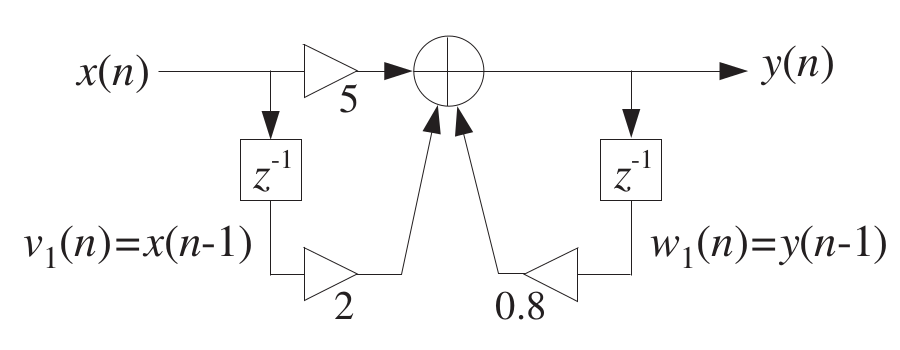
\includegraphics[width=\linewidth]{./picture/direct_form}\newline
	  	$H(z) = \frac{Y(z)}{X(z)} = \frac{5+2z^{-1}}{1-0.8z^{-1}}$ \newline
	  	$Y(z)(1-0.8z^{-1}) = X(z)(5+2z^{-1})$ \newline
	  	$Y(z) = $ \newline $5 X(z) + 2 z^{-1} X(z) + 0.8 z^{-1} Y(z)$
	  		&
	  	  \textbf{canonical form \buchSeite{220}}\newline
	  	  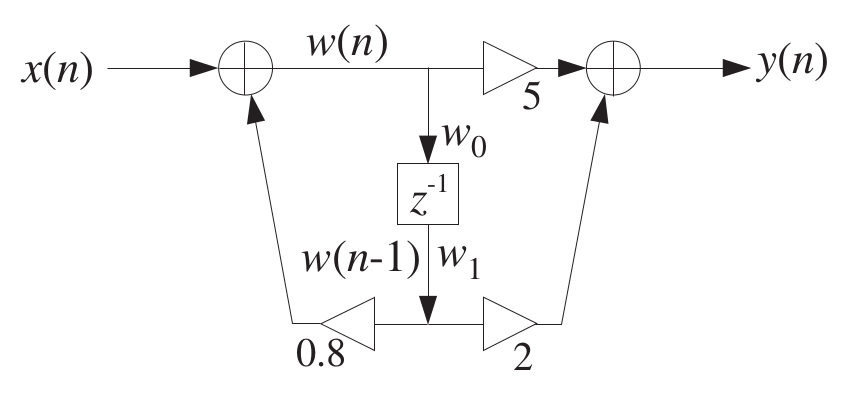
\includegraphics[width=\linewidth]{./picture/canonical_form}
	  	  	$ H(z) = \frac{Y(z)}{X(z)} = \frac{5+2z^{-1}}{1-0.8z^{-1}}$ \newline
	  	  	$ W(z) = \frac{1}{1-0.8z^{-1}} X(z)$ \newline
	  	  	$ W(z) = X(z) + 0.8 z^{-1} W(z)$ \newline
	  	  	$ Y(z) = (5+2z^{-1}) W(z)$
	  	 	&
	  	   \textbf{transposed form \buchSeite{222}}\newline
	  	   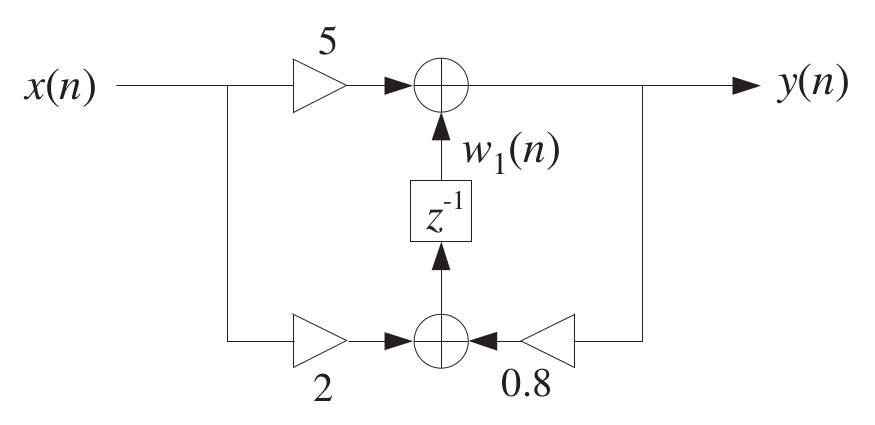
\includegraphics[width=\linewidth]{./picture/transposed_form}\newline
	  	   
%	  	   $W(z) = 2\cdot X(z) + 0.8\cdot Y(z)$\newline
%	  	   $W_1(z) = z^-1 W(z)$\newline
%	  	   $Y(z) = 5\cdot X(z) + Y(z)$\newline??
	  	   
	  	   \textbf{Transposition rules:} \newline
	  	   replace adders by nodes, \newline
	  	   nodes by adders, \newline
	  	   reversing all flows and \newline
	  	   exchanging input with output
\end{longtable}

\subsection{Steady state response\buchSeite{229-232}}
\begin{align*}
  \cos(\omega_0 n) \xrightarrow{H} \left|H(\omega_0) \right| \cos(\omega_0 n + \arg(H(\omega_0))) &&
  \sin(\omega_0 n) \xrightarrow{H} \left|H(\omega_0) \right| \sin(\omega_0 n + \arg(H(\omega_0))) \\
  e^{j\omega_0 n} \xrightarrow{H} H(\omega_0)e^{j\omega_0 n} = |H(\omega_0)| e^{j\omega_0 n + j argH(\omega_0)}
\end{align*}


\begin{tabularx}{0.6\textwidth}{|l|X|}
	\hline
	phase delay & $d(\omega) = - \frac{\arg(H(\omega))}{\omega}$\ \qquad $\arg H(\omega) = -\omega d(\omega)$
	\\ \hline 
	group delay & $d_g(\omega) = -\frac{d}{d\omega}(\arg(H(\omega)))$	
	\\ \hline
\end{tabularx}\\ \\

\subsection{Transient Response\buchSeite{232}}
\begin{tabular}{llll}
  Input sine: &
  $x(n) = e^{j \omega_0 n} \cdot u(n)$ &
  $\Rightarrow$ &
  $X(z) = \frac{1}{1-e^{j \omega_0} z^{-1}}$ \qquad
  ROC $|z| > |e^{j\omega_0}|=1$ \\
  
  time until the output is stable: &
  $n_{eff} = \frac{\ln \epsilon}{\ln \rho} \quad [\text{sample}]$ &
  &
  typ. $\epsilon = 1\%$ \\
 
  &
  $\rho = \max\limits_{i}\left|p_i \right| $ &
  &
  $|p_i|$ is the magnitude of the pole\\
  
  time constant: &
  $\tau = n_{eff}\cdot T$ \\
  
  &
  $H(\omega)=\frac{b}{1-ae^{-j\omega}}$ &
  $\Rightarrow$ &
  $\left| H(\omega)\right| = \frac{b}{\sqrt{1-2a\cos(\omega) + a^2}}$ \\
\end{tabular}

$\left| 1-a e^{-j\omega}\right| = \sqrt{1-2a\cos(\omega) + a^2}$\\

\subsection{Unit Step Response\buchSeite{239}}
\begin{tabularx}{1\textwidth}{l X}
	DC-Gain: & $H(0) = H(z)|_{z=1}= \sum\limits_{n=0}^{\infty}h(n) $
	\\
	AC-Gain: & $H(\pi) = H(z)|_{z=-1}= \sum\limits_{n=0}^{\infty}(-1)^n h(n) $
\end{tabularx}


\subsection{Pole/Zero Design\buchSeite{242-258}}
\subsubsection{First-Order Filters \buchSeite{242}}
  \begin{tabular}{llp{2cm}l}
    Transfer function: &
    $H(z) = \frac{G(1+bz^{-1})}{1-az^{-1}}$ & &
    $a = \epsilon^{1/n_{eff}}$ \\
    $b$ can be calculated from: &
    $\dfrac{H(\pi)}{H(0)} = \dfrac{\text{AC Gain}}{\text{DC Gain}} \left\lbrace \begin{matrix}
      >1 & HP \\
      <1 & LP
    \end{matrix}\right.$ & &
    $a,b \leq 1$ and $G$ = gain
  \end{tabular}

\subsubsection{2 pole conjugate filter\buchSeite{244-246}}

\begin{tabularx}{1\textwidth}{l X}
	poles: & $ p = R e^{j\omega_0}$ \qquad and \qquad $ p^* = R e^{-j\omega_0}$
	\\ 
	Transfer function: & $H(z)= \frac{G}{(1-R e^{-j\omega_0}z^{-1})(1-Re^{j\omega_0}z^{-1})}$\
	$=\frac{G}{1+a_1z^{-1}+a_2z^{-2}}$
	\\
	Parameter: & $a_1 = -2R\cos(\omega_0)$ \qquad; \qquad $a_2 = R^2$
	\\ 
	filter impulse Response & $h(n) = \frac{G}{\sin(\omega_0)}R^n \sin(\omega_0 n + \omega_0)$
	\\ 
	& $G = (1-R)\sqrt{1-2R\cos(2\omega_0)+ R^2}$ \quad only for $|H(\omega_0)| = 1$
\end{tabularx}
\begin{tabularx}{1\textwidth}{Xll}
	3dB width & $\Delta\omega \simeq 2(1-R)$ & $=:R$ is the magnitude of the pole \\
	full width at half maximum of the magnitude squared response & $|H(\omega)|^2=\frac{1}{2}|H(\omega_0)|^2=\frac{1}{2}$&
\end{tabularx}

\subsubsection{2 pole 2 zero filter\buchSeite{228,249}}

\begin{tabular}[b]{l l}
	poles: & $ p = R e^{j\omega_0}$ \qquad and \qquad $ p^* = R e^{-j\omega_0}$
	\\ 
	zeros: & $ z_1 = r e^{j\omega_0}$ \qquad and \qquad $ z_1^* = r e^{-j\omega_0}$
	\\
	Transfer function: & $H(z)= \frac{(1-r e^{j\omega_0}z^{-1})(1-re^{-j\omega_0}z^{-1})}{(1-R e^{j\omega_0}z^{-1})(1-Re^{-j\omega_0}z^{-1})}$\
	$=\frac{1+b_1z^{-1}+b_2z^{-2}}{1+a_1z^{-1}+a_2z^{-2}}$
	\\ 
	Parameter: & $a_1 = -2R\cos(\omega_0)$ \qquad; \qquad $a_2 = R^2$
	\\ 
	& $b_1 = -2r\cos(\omega_0)$ \qquad; \qquad $b_2 = r^2$
\end{tabular}
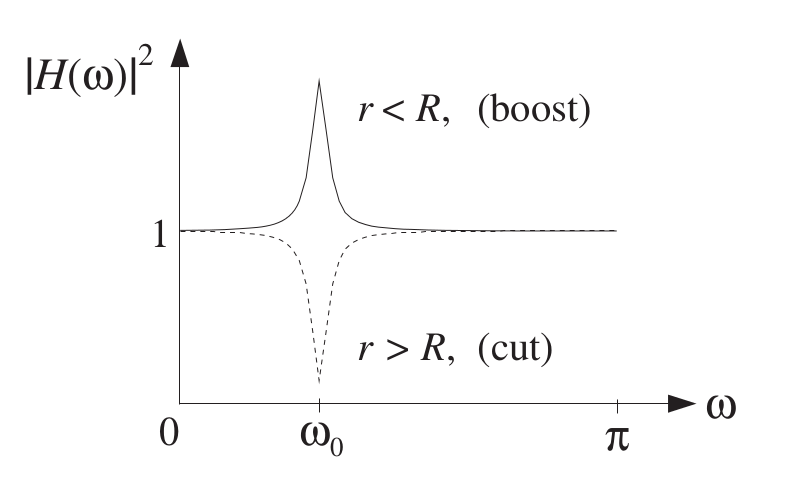
\includegraphics[width=7cm]{./picture/pole_zero_filter}

\subsubsection{Notch and Comb Filter\buchSeite{249-251}}
The zeros of the filters located on the unit circle and the poles are in the unit
circle.

\begin{tabular}{l l}
	Transfer function: & $H(z) = \frac{N(z)}{D(z)} $
	\\
  & $D(z) = N(\rho^{-1}z)  = \prod\limits_{i=1}^{M}(1- e^{j\omega_i}\rho z^{-1)} \qquad \rho$ = Radius	\\
  
  Notch filter:	
	& $N(z) = \prod\limits_{i=1}^{M}(1- e^{j\omega_i}z^{-1)} $ \\
	& $H(z) = \frac{N(z)}{(N\rho^{-1}z)}= \frac{1+b_1 z^{-1} + b_2z^{-2} + \ldots + b_M z^{-M}}
	{1+\rho b_1 z^{-1} + \rho^2 b_2z^{-2} + \ldots + \rho^M b_M z^{-M}} $ \qquad with $0 < |\rho| < 1$\\
	&$a_i=\rho^ib_i \qquad$ mit $\qquad i=1,2,\ldots,M$ \\
	
	Comb filter:
	& $N(z) = \prod\limits_{i=1}^{M}(1- e^{j\omega_i}rz^{-1)} $ \\
	& $H(z) = \frac{N(r^{-1}z)}{N(\rho^{-1}z)} 
	= \frac{1+rb_1z^{-1}+\ldots+r^Mb_Mz^{-M}}{1-\rho b_1z^{-1}+\ldots+\rho^Mb_Mz^{-M}}$ \qquad with $|r| < |\rho| < 1$ 
	\end{tabular}

\newpage	
\subsection{Deconvolution, Inverse Filters and Stability \buchSeite{254-259}}
\begin{multicols}{2}
	\begin{tabular}{ll}
	  & $H_{inv}(z) = \frac{1}{H(z)} = \frac{D(z)}{N(z)}$ \\
	  Deconvolution: &  $x(n) = h_{inv}(n) * y(n)$ \\
	  & $\hat{x}(n) = h_{inv}(n) * y(n) = x(n) + \hat{\nu}(n)$ \\
	  Filtered noise: & $\hat{\nu}(n) = h_{inv}(n) * \nu (n)$
	\end{tabular}\\ \\
	
	$\tilde{h}_{inv}(n) = \left\lbrace\begin{matrix}
    h_{inv}(n) & \text{if } n \geq -D \\
    0 & \text{if } n < -D
  \end{matrix}\right.$ \\

\columnbreak

	Because $H_{inv}(z)$ can have poles outside the unit circle, the stable inverse z-transform $h_{inv}(n)$ will
	necessarily be anticausal. To make a causal system, by clipping of the anticausal tail of the impulse response by a 
	time $n = -D$ and delayed by $D$ time units.\\ \\
	
	$y(n)$ is bounded by some maximal value $|y(n)| \leq A$, so the deconvolution error can be calculated by\\
	$|x(n) - \tilde{x}(n)| \leq A \sum\limits_{m=-\infty}^{-D-1} |h_{inv}(m)|$	
	
\end{multicols}




